\documentclass[]{article}

\usepackage{graphicx}
\usepackage{enumerate}

%opening
\title{structural bioinformatics - assignment 4}
\author{Johanna Becher, Talha Rehman}
\date{}

\begin{document}

\maketitle

\section{Theory exercises}
\subsection{Task 1}
Mutations are changes in a cells genetic information. They can be classified by their formation or by their impact they have. \newline
They can form by insertion or deletion or the change of a single base in the DNA. But it can also happen that a sequence of bases is inserted or deleted.\newline
If the mutation only consists of one base there are diffrent classifications of the mutation depending on the amino acid that is build with the triplet containing the mutation.\newline
A silent mutation occurs when the change of the base doesn't affect the generation of the amino acid at all. A missense mutation leads to a change of the amino acid and a nonsense mutation causes the build in of an early stop codon. \newline

\subsection{Task 2}
Bacteria multiply quite fast by copying it's DNA and dividing into 2 new cells. During the copying mechanism there is a risk that errors occur which would cause a mutation. \newline
Those mutations can have a lethal impact or they can have even no impact at all. But if the mutation causes an adaption of the bacteria to a given condition, due to Darwin's theory of natural selection, it is very propable that this bacteria is going to grow better.\newline
If a bacteria culture is exposed to an antibiotic it could happen, that somme bacteria mutate and their descendants become resistant to this antibiotic.

\subsection{Task 3}

\subsection{Task 4}
We were looking at the protein \textit{TNF-alpha} which is secreted by activated macrophages. It causes the necrosis of tumors (what the name already indicates) but it also plays a role in different signaling pathways.\newline
The top 5 missense mutations are the following:\newline
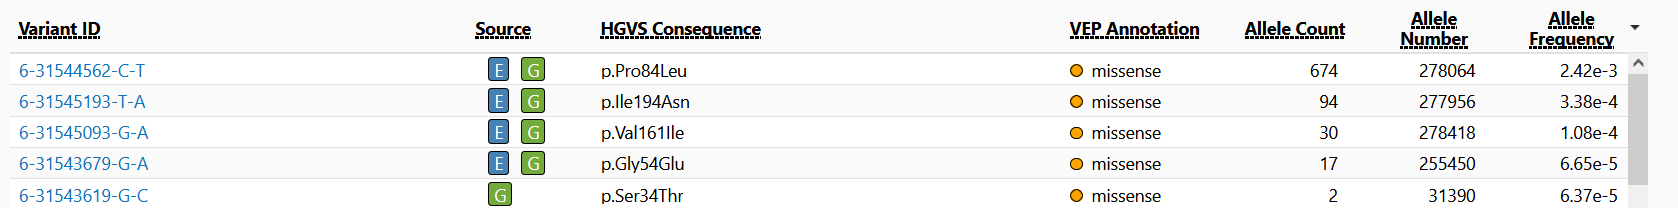
\includegraphics[height=15ex, width=450pt]{mutations.png}
\newline
\newline
In the following picture you see the positions of those 5 mutations marked in red, while the rest of the protein is shown in green.\newline
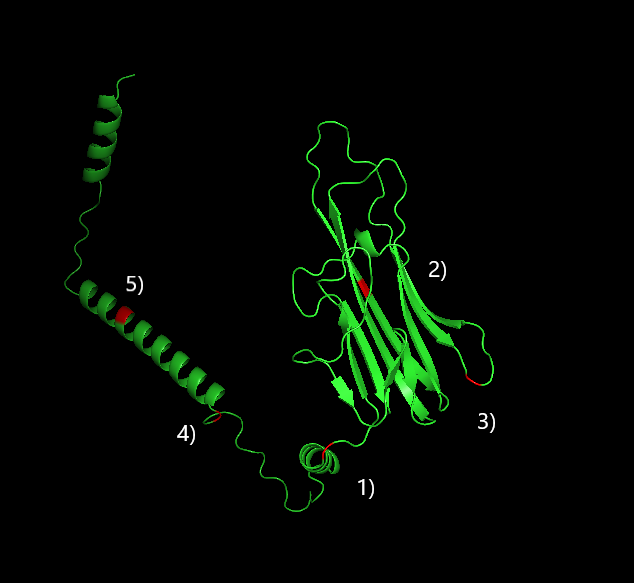
\includegraphics[height=40ex, width=200pt]{mutation_3d_small.png}
\newline
\newline
The numbers indicate the mutations by their allele frequency,
\begin{enumerate}[1)]
	\item position  84: Pro $\rightarrow$ Leu
	\item position 194: Ile $\rightarrow$ Asn
	\item position 161: Val $\rightarrow$ Ile
	\item position  54: Gly $\rightarrow$ Glu
	\item position  34: Ser $\rightarrow$ Thr
\end{enumerate}



\end{document}
